\documentclass[11pt]{article}

\usepackage{amsmath}
\usepackage{amssymb}
\usepackage{booktabs}
\usepackage{graphicx}
\usepackage{hyperref}
\usepackage{natbib}
\usepackage[margin=1in]{geometry}
\usepackage{xcolor}
\usepackage{url}
\usepackage[hyphens]{xurl}
\usepackage{pgfplots}
\pgfplotsset{compat=1.17}

\emergencystretch=1em
\sloppy

\hypersetup{
  colorlinks=true,
  linkcolor=blue,
  citecolor=blue,
  urlcolor=blue
}

\title{Collective Intelligence Peaks at Partial Synchrony:\\
A Coupled-Oscillator Theory of the Diversity--Integration Tradeoff}

\author{
  Philip Phuong Tran\textsuperscript{1}\thanks{Correspondence: Philip Phuong Tran (phil@paragonbiosignals.com)} \\[0.5em]
  \textsuperscript{1} Paragon Biosignals (Univault Technologies LLC), Salt Lake City, Utah, USA
}

\date{}

\begin{document}

\maketitle

\vspace{-1em}

\noindent\textbf{Note on genre.} This is a \emph{theoretical} paper. It introduces no new data. It formalizes, under one dynamical model, a set of results established by others, derives one non-obvious consequence, and states the single pre-registered experiment that would confirm or falsify it. It should be read as a framework and a measurement proposal, not as an empirical study.

\medskip

\noindent\textbf{Competing Interests:} The author is a co-founder and equity holder of Univault Technologies LLC (d/b/a Paragon Biosignals). This work was funded by Univault Technologies LLC. No new human-subjects data were collected; all empirical results discussed are drawn from the cited published literature.

\bigskip

\begin{abstract}
Human groups routinely solve problems that no individual member can, and the effect is measurable rather than metaphorical. We model a group as a network of coupled phase oscillators (the Kuramoto model) whose coupling strength $K$ is set by the \emph{bandwidth and fidelity of information exchange} --- language, shared attention, turn-taking, shared representation --- and not by any physical field. We make one central argument: synchrony is \emph{not} collective intelligence. The Kuramoto order parameter $r$ measures how aligned a group is; but collective intelligence requires both integration (members must pool information) and preserved independence (members must contribute non-redundant information). Using the exact identity from directional statistics that the circular variance of the phase distribution equals $1-r$, we show that a group's collective-intelligence functional is, to leading order, $\mathrm{CI}(r) \propto r\,(1-r)$ --- the product of integration ($r$) and retained diversity ($1-r$) --- and is therefore \emph{unimodal}, peaking at partial synchrony. We tie this functional to the ensemble ambiguity decomposition and the Condorcet jury theorem, and we recover, as a formalization rather than a discovery, the repeatedly observed inverted-U of group performance in coupling: fragmentation at low coupling, groupthink at high. The model yields quantitative, falsifiable predictions: a synchronization onset $r \sim \sqrt{K-K_c}$ near criticality; an optimal coupling $K^\ast$ that \emph{rises} with group diversity (for a diversity scale $\gamma$, the onset is $K_c = 2\gamma$); and coupling graded by channel bandwidth (in-person $>$ video $>$ audio $>$ text). The framework is deliberately bounded --- near-field, channel-mediated, distance-dependent, with no nonlocal term --- and we state the single decisive result, a pre-registered performance peak surviving surrogate-pair controls, that would confirm it or rule it out.

\medskip
\noindent\textbf{Keywords:} collective intelligence, coupled oscillators, Kuramoto model, synchronization, hyperscanning, diversity, wisdom of crowds, groupthink, phase coherence
\end{abstract}

\section{The phenomenon to be explained}

Groups routinely outperform their members. A committee, a research team, a jury, or a crowd can reach conclusions that none of its individuals could reach alone, and the effect is measurable: the collective-intelligence factor of a group correlates only weakly with the average or peak intelligence of its members \citep{woolley2010evidence}. Two standard accounts of this fact both fail.

The \emph{deflationary} account holds that a group merely averages or aggregates individual ability, so collective performance is a simple function of member IQ. This is empirically false: the group $c$-factor tracks features of the interaction --- social sensitivity, equality of turn-taking --- rather than the members' individual scores \citep{woolley2010evidence}.

The \emph{inflationary} account posits a coupling field or shared medium that links minds directly. In its strongest, planetary-scale form this account is not merely unsupported but physically untenable, and we do not defend it here.\footnote{An earlier formulation by the present author proposed that inter-individual coupling was mediated by a planetary physical medium (geomagnetic and Schumann-band resonance). That claim is withdrawn on physical grounds: the power a warm-bodied biological source can inject into a planetary cavity mode is many orders of magnitude below the lightning-driven background that already saturates it, and the required persistent coherence is incompatible with thermal scales. The present framework retains none of that mechanism. It is included here only to disclose the intellectual provenance of the ``coherence'' vocabulary.}

The correct account sits between the two. Collective intelligence is a genuine emergent property of a \emph{coupled network}, but the coupling runs through an ordinary, extraordinarily high-bandwidth channel --- sensory and linguistic exchange --- not through a field. The intelligence is real; the medium is air, light, and language. The mechanism of inter-individual coupling in this sense --- brain-to-brain coupling through the shared physical world --- was framed by \citet{hasson2012brain}, and speaker--listener neural coupling that tracks the success of communication was demonstrated by \citet{stephens2010speaker}. Our contribution is not to discover this coupling but to give it a dynamical formalism, and to extract from that formalism one prediction the existing literature does not state: \emph{where}, quantitatively, collective intelligence should peak as a function of coupling and diversity.

\section{A coupled-oscillator model of interacting minds}

\subsection{The dynamics}

Represent each of $N$ interacting individuals $i$ as a phase oscillator with phase $\theta_i$ and intrinsic frequency $\omega_i$, the latter capturing that individual's characteristic cognitive/physiological tempo and disposition. Neural, cardiac, and respiratory activity is rhythmic and entrainable, and inter-brain and inter-physiological rhythms phase-align during interaction to a degree that tracks the quality of that interaction \citep{stephens2010speaker, dikker2017brain}. The canonical mean-field dynamics for such a system is the Kuramoto model \citep{kuramoto1984chemical, strogatz2000kuramoto}:
\begin{equation}
\frac{d\theta_i}{dt} = \omega_i + \frac{K}{N}\sum_{j=1}^{N}\sin(\theta_j - \theta_i).
\label{eq:kuramoto}
\end{equation}
The collective state is summarized by the complex order parameter
\begin{equation}
r\,e^{i\psi} = \frac{1}{N}\sum_{j=1}^{N} e^{i\theta_j}, \qquad r \in [0,1],
\label{eq:order}
\end{equation}
where $r$ measures group synchrony: $r \to 0$ is incoherence, $r \to 1$ is full phase-locking.

The one substantive interpretive move is that $K$ here is \emph{not} a physical field coupling. It is a phenomenological coupling constant standing for the bandwidth and fidelity of information exchange between members: the rate and accuracy with which one member's state can influence another's. High-bandwidth, high-trust, well-structured interaction is large $K$; degraded, low-trust, or channel-impaired interaction is small $K$. We treat bandwidth as a monotone proxy for $K$ and do not claim to derive the sinusoidal coupling form from a communication channel; the sine term is the standard weak-coupling phase reduction \citep{pikovsky2001synchronization}, and $K$ is the phenomenological coupling it leaves behind.

\subsection{Diversity sets the synchronization threshold}

For a distribution of intrinsic frequencies $g(\omega)$ with a characteristic half-width $\gamma$ --- the heterogeneity of members' dispositions, which we call \emph{viewpoint diversity} --- the mean-field theory gives a critical coupling for the onset of synchronization \citep{kuramoto1984chemical, strogatz2000kuramoto, acebron2005kuramoto},
\begin{equation}
K_c = \frac{2}{\pi\,g(0)}.
\end{equation}
For the analytically tractable Lorentzian $g(\omega) = (\gamma/\pi)/(\omega^2 + \gamma^2)$, one has $g(0) = 1/(\pi\gamma)$, so
\begin{equation}
K_c = 2\gamma.
\label{eq:kc}
\end{equation}
More diverse groups (larger $\gamma$) require stronger coupling --- better communication --- to integrate at all. This is the right qualitative structure: the same parameter that governs whether a group coheres also encodes how much independent variation it carries. Two caveats are important and are treated honestly rather than hidden. First, the Lorentzian is chosen for tractability (it has infinite variance, so $\gamma$ is a scale parameter, not a standard deviation); nothing in the argument requires dispositions to be Cauchy-distributed, and $\gamma$ should be read as a heterogeneity scale. Second, Eq.~\eqref{eq:kc} is a mean-field, all-to-all, $N\to\infty$ result; real groups are small, sparsely and directionally connected. On a network with adjacency matrix $A$, the threshold instead scales as $K_c \propto 1/\lambda_{\max}(A)$, the inverse of the largest eigenvalue \citep{restrepo2005onset}. We return to finite $N$ and network structure in Section~\ref{sec:scope}.

\subsection{Near the onset}

The Kuramoto model makes a sharper, more distinctive prediction than a threshold alone. For a symmetric unimodal $g$, synchronization emerges through a supercritical bifurcation, and just above onset the order parameter grows as \citep{strogatz2000kuramoto, acebron2005kuramoto}
\begin{equation}
r \sim \sqrt{K - K_c}.
\label{eq:sqrt}
\end{equation}
This square-root law is a fingerprint of the specific $\sin(\theta_j-\theta_i)$ coupling; a generic ``coupling increases with channel quality'' model does not produce it. Eq.~\eqref{eq:sqrt}, and its rounding at finite $N$, is therefore the measurement that would distinguish genuine coupled-oscillator dynamics from a mere monotone association between communication and synchrony. We flag it as the model's most falsifiable claim.

\section{Why synchrony is not collective intelligence}

\subsection{The integration--independence tradeoff}

Synchrony $r$ is not collective intelligence. A perfectly synchronized group ($r \to 1$) is one in which every member has become a copy of every other; diversity has collapsed. Collective intelligence requires \emph{both} integration (members must pool information) \emph{and} preserved independence (members must contribute non-redundant information).

This is not a soft intuition; it is the content of two exact results. The \emph{ensemble ambiguity decomposition} \citep{krogh1995neural} states that the error of an averaged ensemble equals the average member error minus the diversity of member errors:
\begin{equation}
E_{\text{collective}} = \bar{E}_{\text{member}} - \bar{A}_{\text{ambiguity}}.
\label{eq:ambiguity}
\end{equation}
Collective performance improves with member competence \emph{and} with diversity; the same point, for prediction, is Page's diversity result \citep{hong2004groups}. From the other direction, the Condorcet jury theorem \citep{condorcet1785essai} shows that a group's aggregate judgment beats the individual's only when member judgments are \emph{independent}. Coupling that drives members into agreement destroys exactly the independence these results require.

\subsection{The functional, derived rather than posited}

We want a functional that expresses collective intelligence as (integration) $\times$ (retained independence) in terms of the state variable of the dynamics. Integration is captured directly by the order parameter $r$. Retained independence is captured by the dispersion of the phase distribution. Here we use an exact identity from directional statistics: the \emph{circular variance} of a set of phases is \citep{mardia2000directional}
\begin{equation}
V = 1 - r.
\end{equation}
That is, $1-r$ is not a heuristic stand-in for diversity; it \emph{is} the circular variance of the group's phase distribution. Taking collective intelligence to leading order as the product of integration and retained dispersion gives
\begin{equation}
\boxed{\;\mathrm{CI}(r) \;\propto\; \underbrace{r}_{\text{integration}} \cdot \underbrace{(1-r)}_{\text{retained independence}}\;}
\label{eq:ci}
\end{equation}
which is unimodal in $r$, rising from zero at $r=0$ (fragmentation), peaking at partial synchrony, and returning to zero at $r=1$ (redundancy) (Fig.~\ref{fig:ci}). We state plainly what Eq.~\eqref{eq:ci} is and is not. It is the leading-order functional consistent with the ambiguity decomposition and with the circular-variance identity: the lowest-order product of an integration term that must vanish at $r=0$ and an independence term that must vanish at $r=1$. It is \emph{not} claimed to be the exact collective-intelligence function; the true functional --- in particular the location of the peak, which the symmetric form places at $r=1/2$ --- is an empirical quantity to be estimated, and a full derivation from the phase-density dynamics (e.g.\ via the Ott--Antonsen reduction for a Lorentzian $g$ \citep{ott2008low}) is left to future work. The claim we defend is the \emph{unimodality} and its origin in the integration--independence tradeoff, not the precise algebraic form.

\begin{figure}[ht]
\centering
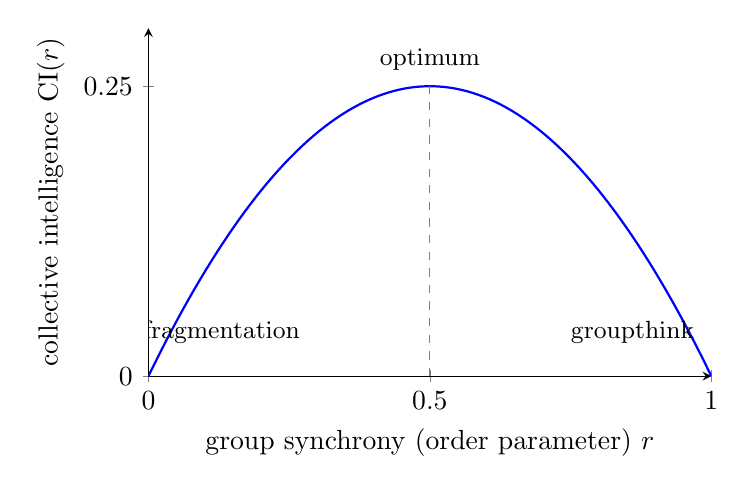
\begin{tikzpicture}
\begin{axis}[
  width=0.72\textwidth, height=6cm,
  xlabel={group synchrony (order parameter) $r$},
  ylabel={collective intelligence $\mathrm{CI}(r)$},
  xmin=0, xmax=1, ymin=0, ymax=0.30,
  samples=100, domain=0:1,
  axis lines=left, xtick={0,0.5,1}, ytick={0,0.25},
  every axis plot/.append style={thick}
]
\addplot[blue, thick] {x*(1-x)};
\draw[gray, dashed] (axis cs:0.5,0) -- (axis cs:0.5,0.25);
\node[anchor=south] at (axis cs:0.13,0.02) {\small fragmentation};
\node[anchor=south] at (axis cs:0.86,0.02) {\small groupthink};
\node[anchor=south] at (axis cs:0.5,0.255) {\small optimum};
\end{axis}
\end{tikzpicture}
\caption{The integration--independence tradeoff. Collective intelligence is unimodal in group synchrony $r$ because it is the product of an integration term $r$ and a retained-independence term $1-r$ (the circular variance of the phase distribution). Low coupling leaves the group fragmented; high coupling collapses independence into groupthink. The symmetric leading-order form $\mathrm{CI}\propto r(1-r)$ places the optimum at $r=1/2$; the true peak location is an empirical quantity.}
\label{fig:ci}
\end{figure}

\subsection{Two failure modes, and a known result formalized}

The functional names two failure modes, both independently documented:
\begin{itemize}
  \item \textbf{Under-coupling} ($r \to 0$, $K < K_c$): members never integrate; the group is a disconnected set. Fragmentation.
  \item \textbf{Over-coupling} ($r \to 1$, $K \gg K_c$): independence collapses; the group becomes one redundant voice. Groupthink.
\end{itemize}
We emphasize that the inverted-U itself is \emph{not new}. It is one of the most robust findings in the study of groups, and our contribution is to formalize it, not to discover it. Efficient, highly connected communication networks converge prematurely on inferior solutions while inefficient networks preserve diversity and end up smarter \citep{lazer2007network}; intermittent breaks in interaction --- intermediate coupling --- improve collective intelligence over constant interaction \citep{bernstein2018intermittent}; and social influence narrows the diversity of estimates, degrading accuracy while inflating confidence \citep{lorenz2011social}. Network structure determines whether influence helps or harms crowd wisdom \citep{becker2017network}. Eq.~\eqref{eq:ci} is a compact dynamical statement of what these studies observe. Its value, if any, is not the observation but the quantitative link it draws to a measurable coupling $K$, a measurable synchrony $r$, and a measurable diversity $\gamma$.

\section{Predictions and the decisive test}

Each prediction is stated with the observation that would refute it.

\begin{enumerate}
  \item \textbf{Synchronization onset.} Near criticality, group synchrony grows as $r \sim \sqrt{K-K_c}$ (Eq.~\ref{eq:sqrt}), with characteristic finite-$N$ rounding. \emph{Refuted by}: a linear or thresholdless $r(K)$ across graded coupling.
  \item \textbf{The inverted-U, with an a-priori peak.} Group task performance is non-monotone in measured synchrony $r$, rising then falling. The falsifiable, pre-registrable form: specify the predicted peak location $r^\ast$ and effect size \emph{before} data collection; the model is refuted if performance is monotone in $r$, or if the peak lies outside the pre-registered interval, once the estimate is required to exceed a surrogate-pair null (Section~\ref{sec:measure}). This replaces vague ``an optimum exists somewhere'' with a committed number.
  \item \textbf{Diversity raises the optimum.} The coupling at which performance peaks, $K^\ast$, increases with viewpoint diversity $\gamma$ (Eq.~\ref{eq:kc}): diverse teams require richer communication to reach the same integration. \emph{Refuted by}: an optimal coupling independent of, or decreasing with, measured group diversity.
  \item \textbf{Bandwidth grading.} Coupling, and inter-brain/inter-physiological synchrony up to the optimum, increase with channel bandwidth: in-person $>$ full video $>$ audio-only $>$ text-only. \emph{Caveat}: bandwidth co-varies with arousal and stimulus richness, which must be controlled. \emph{Refuted by}: no ordering of coupling by channel bandwidth.
  \item \textbf{Directionality.} Coupling is directed and asymmetric (leaders/teachers drive followers/learners), detectable via transfer entropy \citep{schreiber2000measuring} or convergent cross-mapping \citep{sugihara2012detecting}, not merely symmetric coherence. \emph{Refuted by}: purely symmetric coupling in structured leader--follower interactions.
\end{enumerate}

The predictions that carry the theory are (2) and (3): a quantitatively located, diversity-dependent performance optimum. Prediction (1) certifies that the dynamics are genuinely of Kuramoto type rather than a generic monotone coupling.

\section{Measurement}
\label{sec:measure}

\paragraph{The common-driver problem is the central methodological hazard.} Two people attending to the same time-locked stimulus will show correlated physiology with \emph{no} interaction-specific coupling between them, and, because their individual response latencies differ, this shared drive manufactures precisely the lagged, asymmetric signatures --- directed transfer entropy, non-zero imaginary coherence --- that one might otherwise nominate as evidence of coupling \citep{burgess2013conceptual, novembre2021hyperscanning, hamilton2021hyperscanning}. Directionality and lag analysis alone therefore do \emph{not} establish inter-individual coupling. The load-bearing control must be a \textbf{surrogate-pair (pseudo-hyperscanning) null}: coupling is recomputed on non-interacting members shuffled across dyads, and a genuine coupling estimate must exceed this partner-shuffled distribution. Interacting-versus-silent-co-presence contrasts and phase-randomized surrogates are secondary controls. No synchrony number in this program is interpretable without the surrogate-pair null stated as its primary comparison.

\paragraph{Coupling metrics.} We use standard, published, reproducible estimators: phase-locking value, the imaginary part of coherency to suppress volume-conduction and shared-reference artifacts \citep{nolte2004identifying}, transfer entropy \citep{schreiber2000measuring}, and convergent cross-mapping \citep{sugihara2012detecting}. Where a common latent space across individuals is desired --- so that coupling is computed on comparable representations rather than raw idiosyncratic signals --- this is the hyperalignment / shared-response-model problem \citep{haxby2011common, chen2015reduced}, and any subject-invariant encoder used should be reported as an adaptation of those methods, validated on held-out subjects, and, ideally, open, so the program is reproducible without proprietary components.

\paragraph{Design and standards.} Co-located dyads and small groups, within-subject, across graded communication conditions and graded diversity; pre-registered protocols and analysis plans; analyst blinding; permutation and cluster-based inference with multiple-comparison correction; effect sizes and confidence intervals reported; independent replication required before any claim. A defensible first study need not collect new data at all: a re-analysis of an existing open hyperscanning dataset \citep{dikker2017brain}, with a pre-registered $r^\ast$ and the surrogate-pair null, would test prediction (2) directly.

\section{Scope, boundary, and a note on scale}
\label{sec:scope}

The strength of this framework is its boundary. It claims that coupling is informational and near-field, that correlations are distance-dependent and decay with channel degradation, and that there is no nonlocal correlation, no distance-independent term, and no planetary or cosmic medium. Anything beyond this boundary is outside the theory.

Two internal limits are stated honestly. First, \textbf{finite $N$}: the phase transition and $K_c = 2\gamma$ are $N\to\infty$ results, whereas real groups and the dyads of any feasible experiment have $N \sim 2$--$10$, where there is no sharp transition and $r$ fluctuates at order $1/\sqrt{N}$. The small-$N$ predictions are therefore best framed as finite-size scaling --- how the optimum and the $c$-factor trend with group size --- rather than as a critical threshold. Second, \textbf{topology}: Eq.~\eqref{eq:kuramoto} is all-to-all, which has no structure, in tension with the claim that intelligence lives in the interaction structure. A network Kuramoto model, with $K_c$ set by $\lambda_{\max}(A)$ \citep{restrepo2005onset} and directed coupling consistent with prediction (5), is the natural and more honest next step, and connects the framework to the collective-intelligence literature on network structure \citep{lazer2007network, becker2017network}.

Finally, a single scale remark, offered as a hypothesis and not a result: the same over-coupling that produces groupthink in a team would, in a decentralized decision system, produce false convergence --- agreement that carries no information because the independence that made agreement informative was destroyed. Whether collective intelligence and convergence-based collective decision-making are the same theory at two scales is a question this framework raises but does not settle; establishing it would require a cross-scale invariant that is not estimated here.

\section{Conclusion}

Human groups are coupled networks, and the coupling that joins two minds in a conversation is, we argue, the same coupling --- through language, attention, and shared representation --- that lets a group think past its members. Modeling that coupling as a Kuramoto system makes one thing precise that the prior literature leaves qualitative: collective intelligence is not synchrony but the product of synchrony and retained diversity, $\mathrm{CI} \propto r(1-r)$, and it therefore peaks at partial synchrony, at a coupling that rises with the group's diversity. That is a formalization of a well-established inverted-U, not a new empirical claim; its worth will be decided by whether a pre-registered, diversity-dependent performance optimum, located a priori and defended against a surrogate-pair null, survives contact with data. The framework is smaller than the intuition that motivated it --- it makes no claim to a field, a medium, or a nonlocal bond --- and it is stronger for the reduction.

\bigskip

\noindent\textbf{Data and code availability.} This is a theoretical paper; it generates no new data. The figure is produced by the equation $\mathrm{CI}(r)=r(1-r)$ and requires no data.

\bigskip

\bibliographystyle{plainnat}

\begin{thebibliography}{99}

\bibitem[Acebr{\'o}n et~al.(2005)]{acebron2005kuramoto}
J.~A.~Acebr{\'o}n, L.~L.~Bonilla, C.~J.~P{\'e}rez~Vicente, F.~Ritort, and R.~Spigler.
\newblock The Kuramoto model: A simple paradigm for synchronization phenomena.
\newblock \emph{Reviews of Modern Physics}, 77(1):137--185, 2005.

\bibitem[Becker et~al.(2017)]{becker2017network}
J.~Becker, D.~Brackbill, and D.~Centola.
\newblock Network dynamics of social influence in the wisdom of crowds.
\newblock \emph{Proceedings of the National Academy of Sciences}, 114(26):E5070--E5076, 2017.

\bibitem[Bernstein et~al.(2018)]{bernstein2018intermittent}
E.~Bernstein, J.~Shore, and D.~Lazer.
\newblock How intermittent breaks in interaction improve collective intelligence.
\newblock \emph{Proceedings of the National Academy of Sciences}, 115(35):8734--8739, 2018.

\bibitem[Burgess(2013)]{burgess2013conceptual}
A.~P.~Burgess.
\newblock On the interpretation of synchronization in EEG hyperscanning studies: a cautionary note.
\newblock \emph{Frontiers in Human Neuroscience}, 7:881, 2013.

\bibitem[Chen et~al.(2015)]{chen2015reduced}
P.~H.~Chen, J.~Chen, Y.~Yeshurun, U.~Hasson, J.~Haxby, and P.~J.~Ramadge.
\newblock A reduced-dimension fMRI shared response model.
\newblock In \emph{Advances in Neural Information Processing Systems}, vol.~28, 2015.

\bibitem[Condorcet(1785)]{condorcet1785essai}
Marquis de Condorcet.
\newblock \emph{Essai sur l'application de l'analyse {\`a} la probabilit{\'e} des d{\'e}cisions rendues {\`a} la pluralit{\'e} des voix}.
\newblock Imprimerie Royale, Paris, 1785.

\bibitem[Dikker et~al.(2017)]{dikker2017brain}
S.~Dikker, L.~Wan, I.~Davidesco, L.~Kaggen, M.~Oostrik, J.~McClintock, J.~Rowland, G.~Michalareas, J.~J.~Van~Bavel, M.~Ding, and D.~Poeppel.
\newblock Brain-to-brain synchrony tracks real-world dynamic group interactions in the classroom.
\newblock \emph{Current Biology}, 27(9):1375--1380, 2017.

\bibitem[Hamilton(2021)]{hamilton2021hyperscanning}
A.~F.~de~C.~Hamilton.
\newblock Hyperscanning: Beyond the hype.
\newblock \emph{Neuron}, 109(3):404--407, 2021.

\bibitem[Hasson et~al.(2012)]{hasson2012brain}
U.~Hasson, A.~A.~Ghazanfar, B.~Galantucci, S.~Garrod, and C.~Keysers.
\newblock Brain-to-brain coupling: a mechanism for creating and sharing a social world.
\newblock \emph{Trends in Cognitive Sciences}, 16(2):114--121, 2012.

\bibitem[Haxby et~al.(2011)]{haxby2011common}
J.~V.~Haxby, J.~S.~Guntupalli, A.~C.~Connolly, Y.~O.~Halchenko, B.~R.~Conroy, M.~I.~Gobbini, M.~Hanke, and P.~J.~Ramadge.
\newblock A common, high-dimensional model of the representational space in human ventral temporal cortex.
\newblock \emph{Neuron}, 72(2):404--416, 2011.

\bibitem[Hong and Page(2004)]{hong2004groups}
L.~Hong and S.~E.~Page.
\newblock Groups of diverse problem solvers can outperform groups of high-ability problem solvers.
\newblock \emph{Proceedings of the National Academy of Sciences}, 101(46):16385--16389, 2004.

\bibitem[Krogh and Vedelsby(1995)]{krogh1995neural}
A.~Krogh and J.~Vedelsby.
\newblock Neural network ensembles, cross validation, and active learning.
\newblock In \emph{Advances in Neural Information Processing Systems}, vol.~7, pp.~231--238, 1995.

\bibitem[Kuramoto(1984)]{kuramoto1984chemical}
Y.~Kuramoto.
\newblock \emph{Chemical Oscillations, Waves, and Turbulence}.
\newblock Springer, Berlin, 1984.

\bibitem[Lazer and Friedman(2007)]{lazer2007network}
D.~Lazer and A.~Friedman.
\newblock The network structure of exploration and exploitation.
\newblock \emph{Administrative Science Quarterly}, 52(4):667--694, 2007.

\bibitem[Lorenz et~al.(2011)]{lorenz2011social}
J.~Lorenz, H.~Rauhut, F.~Schweitzer, and D.~Helbing.
\newblock How social influence can undermine the wisdom of crowd effect.
\newblock \emph{Proceedings of the National Academy of Sciences}, 108(22):9020--9025, 2011.

\bibitem[Mardia and Jupp(2000)]{mardia2000directional}
K.~V.~Mardia and P.~E.~Jupp.
\newblock \emph{Directional Statistics}.
\newblock Wiley, Chichester, 2000.

\bibitem[Nolte et~al.(2004)]{nolte2004identifying}
G.~Nolte, O.~Bai, L.~Wheaton, Z.~Mari, S.~Vorbach, and M.~Hallett.
\newblock Identifying true brain interaction from EEG data using the imaginary part of coherency.
\newblock \emph{Clinical Neurophysiology}, 115(10):2292--2307, 2004.

\bibitem[Novembre and Iannetti(2021)]{novembre2021hyperscanning}
G.~Novembre and G.~D.~Iannetti.
\newblock Hyperscanning alone cannot prove causality. Multibrain stimulation can.
\newblock \emph{Trends in Cognitive Sciences}, 25(2):96--99, 2021.

\bibitem[Ott and Antonsen(2008)]{ott2008low}
E.~Ott and T.~M.~Antonsen.
\newblock Low dimensional behavior of large systems of globally coupled oscillators.
\newblock \emph{Chaos}, 18(3):037113, 2008.

\bibitem[Pikovsky et~al.(2001)]{pikovsky2001synchronization}
A.~Pikovsky, M.~Rosenblum, and J.~Kurths.
\newblock \emph{Synchronization: A Universal Concept in Nonlinear Sciences}.
\newblock Cambridge University Press, Cambridge, 2001.

\bibitem[Restrepo et~al.(2005)]{restrepo2005onset}
J.~G.~Restrepo, E.~Ott, and B.~R.~Hunt.
\newblock Onset of synchronization in large networks of coupled oscillators.
\newblock \emph{Physical Review E}, 71(3):036151, 2005.

\bibitem[Schreiber(2000)]{schreiber2000measuring}
T.~Schreiber.
\newblock Measuring information transfer.
\newblock \emph{Physical Review Letters}, 85(2):461--464, 2000.

\bibitem[Stephens et~al.(2010)]{stephens2010speaker}
G.~J.~Stephens, L.~J.~Silbert, and U.~Hasson.
\newblock Speaker--listener neural coupling underlies successful communication.
\newblock \emph{Proceedings of the National Academy of Sciences}, 107(32):14425--14430, 2010.

\bibitem[Strogatz(2000)]{strogatz2000kuramoto}
S.~H.~Strogatz.
\newblock From Kuramoto to Crawford: exploring the onset of synchronization in populations of coupled oscillators.
\newblock \emph{Physica D}, 143(1--4):1--20, 2000.

\bibitem[Sugihara et~al.(2012)]{sugihara2012detecting}
G.~Sugihara, R.~May, H.~Ye, C.~H.~Hsieh, E.~Deyle, M.~Fogarty, and S.~Munch.
\newblock Detecting causality in complex ecosystems.
\newblock \emph{Science}, 338(6106):496--500, 2012.

\bibitem[Woolley et~al.(2010)]{woolley2010evidence}
A.~W.~Woolley, C.~F.~Chabris, A.~Pentland, N.~Hashmi, and T.~W.~Malone.
\newblock Evidence for a collective intelligence factor in the performance of human groups.
\newblock \emph{Science}, 330(6004):686--688, 2010.

\end{thebibliography}

\end{document}
